\chapter{xm}

\begin{figure}[h!]
\centering
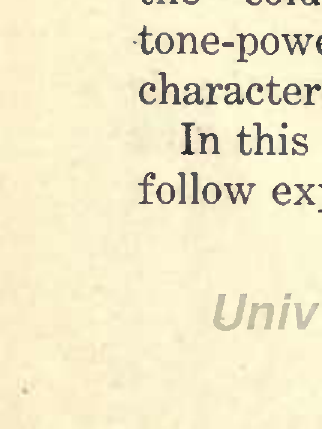
\includegraphics[width=0.8\textwidth]{../imagenes/pagina_022_fig_01.png}
\caption{Figura de la página 22}
\end{figure}

\begin{figure}[h!]
\centering
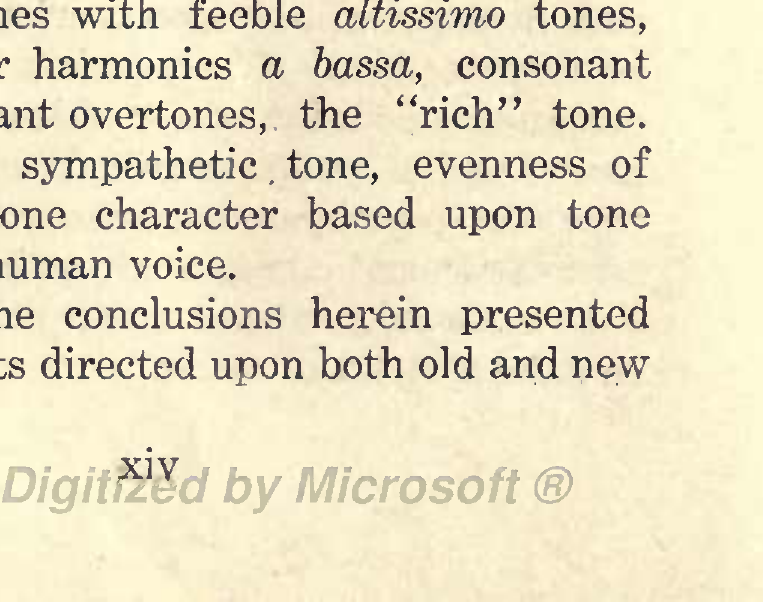
\includegraphics[width=0.8\textwidth]{../imagenes/pagina_022_fig_02.png}
\caption{Figura de la página 22}
\end{figure}

\begin{figure}[h!]
\centering
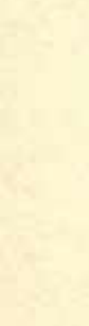
\includegraphics[width=0.8\textwidth]{../imagenes/pagina_022_fig_03.png}
\caption{Figura de la página 22}
\end{figure}

\begin{figure}[h!]
\centering
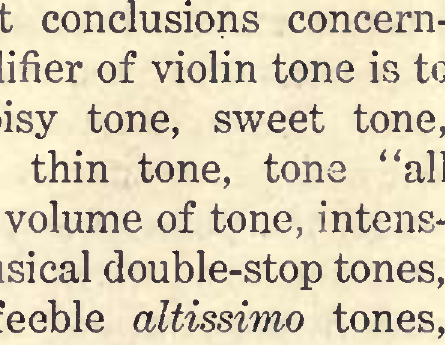
\includegraphics[width=0.8\textwidth]{../imagenes/pagina_022_fig_04.png}
\caption{Figura de la página 22}
\end{figure}

\begin{figure}[h!]
\centering
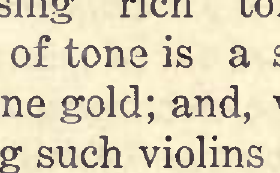
\includegraphics[width=0.8\textwidth]{../imagenes/pagina_022_fig_05.png}
\caption{Figura de la página 22}
\end{figure}

\begin{figure}[h!]
\centering
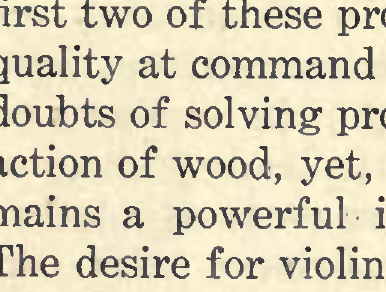
\includegraphics[width=0.8\textwidth]{../imagenes/pagina_022_fig_06.png}
\caption{Figura de la página 22}
\end{figure}

\begin{figure}[h!]
\centering
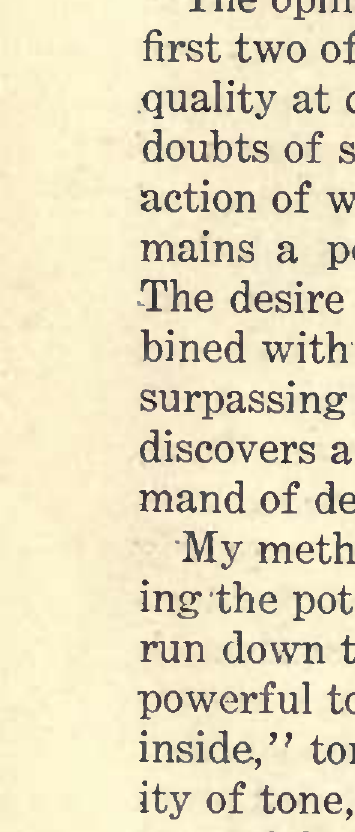
\includegraphics[width=0.8\textwidth]{../imagenes/pagina_022_fig_07.png}
\caption{Figura de la página 22}
\end{figure}

\begin{figure}[h!]
\centering
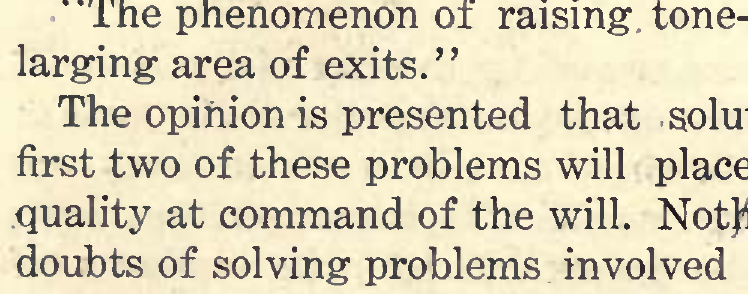
\includegraphics[width=0.8\textwidth]{../imagenes/pagina_022_fig_08.png}
\caption{Figura de la página 22}
\end{figure}

\begin{figure}[h!]
\centering
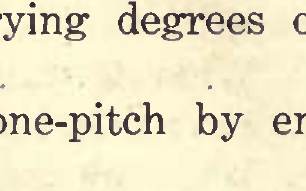
\includegraphics[width=0.8\textwidth]{../imagenes/pagina_022_fig_09.png}
\caption{Figura de la página 22}
\end{figure}

\begin{figure}[h!]
\centering
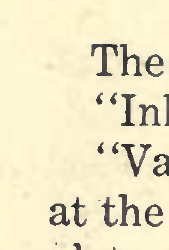
\includegraphics[width=0.8\textwidth]{../imagenes/pagina_022_fig_10.png}
\caption{Figura de la página 22}
\end{figure}

\begin{figure}[h!]
\centering
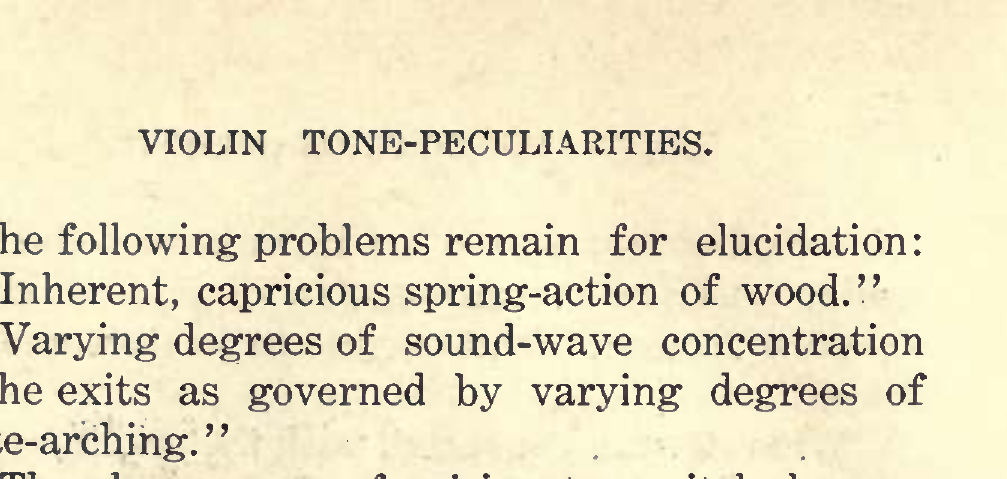
\includegraphics[width=0.8\textwidth]{../imagenes/pagina_022_fig_11.png}
\caption{Figura de la página 22}
\end{figure}

\begin{figure}[h!]
\centering
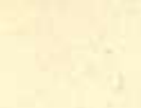
\includegraphics[width=0.8\textwidth]{../imagenes/pagina_022_fig_12.png}
\caption{Figura de la página 22}
\end{figure}

\section{VIOLIN TONE-PECULIARITIES.}

The following problems remain for elucidation: ' 'Inherent, capricious spring-action of wood. ' ' ' 'Varying degrees of sound-wave concentration at the exits as governed by varying degrees of plate-arching." 'The ' phenomenon of raising tone-pitch by en- larging area of exits." The opinion is presented that solutions for the first two of these problems will place violin tone- quality at command of the will. Notwithstanding doubts of solving problems involved in capricious action of wood, yet, the value in such solution re- mains a powerful incentive to continued effort. The desire for violins possessing "rich" tone com- bined with marked intensity of tone is a stimulus surpassing the stimulus of fine gold; and, whoever discovers a method producing such violins at com- mand of desire will become a king in his own right. My method for arriving at conclusions concern- ing the potency in each modifier of violin tone is to run down the causes for noisy tone, sweet tone, powerful tone, hollow tone, thin tone, tone "all inside," tone "all outside," volume of tone, intens- ity of tone, tone pitch, unmusical double-stop tones, powerful open tones with feeble altissimo tones, resultant tones, or harmonics a bassa, consonant overtones, dissonant overtones, the "rich" tone, the "cold" tone, sympathetic tone, evenness of tone-power, and tone character . based upon tone character of the human voice. In this work, the conclusions herein presented follow experiments directed upon both old and new

\section{xiv}

\begin{figure}[h!]
\centering
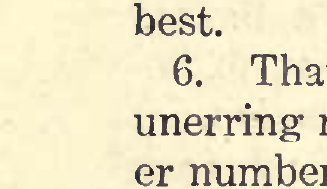
\includegraphics[width=0.8\textwidth]{../imagenes/pagina_023_fig_01.png}
\caption{Figura de la página 23}
\end{figure}

\begin{figure}[h!]
\centering
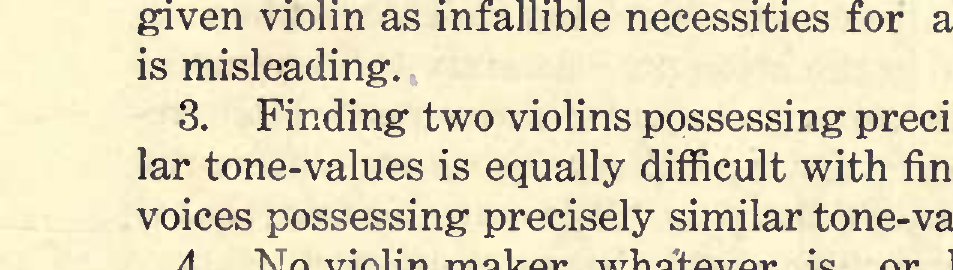
\includegraphics[width=0.8\textwidth]{../imagenes/pagina_023_fig_02.png}
\caption{Figura de la página 23}
\end{figure}

\begin{figure}[h!]
\centering
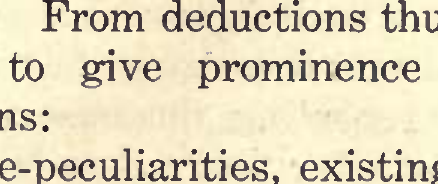
\includegraphics[width=0.8\textwidth]{../imagenes/pagina_023_fig_03.png}
\caption{Figura de la página 23}
\end{figure}

\section{VIOLIN TONE-PECULIARITIES.}

violins, and the number of such violins runs into hundreds. From deductions thus obtained, it is my desire to give prominence to the following propositions: 1. Tone-peculiarities, existing in. a given violin, may not exist in any other violin. 2. Writing up tone-peculiarities existing in a given violin as infallible necessities for all violins is misleading. 3. Finding two violins possessing precisely simi- lar tone- values is equally difficult with finding two voices possessing precisely similar tone- values. 4. No violin maker whatever, is, or has been able to give marked tone- value to each and every violin. 5. That the mountain herder of sheep may pro- duce a violin possessing tone-values equal to the best. 6. That th3 skillful mechanic, guided by unerring musical instinct, produces a vastly great- er number of superior violins than the mechanic minus such instinct. 7. That all .violin makers may meet occasional defeat. 8. That, barring accident, the superior violin is a product of superior mechanical skill combined with superior musical sense, all being directed up- on superior material. Than the method herein presented for determin- ing the potency and operation of each factor enter- ing into the production and modification of violin tone, there seems no other method offering equal

\section{xv}

\begin{figure}[h!]
\centering

\includegraphics[width=0.8\textwidth]{../imagenes/pagina_024_fig_01.png}
\caption{Figura de la página 24}
\end{figure}

\begin{figure}[h!]
\centering
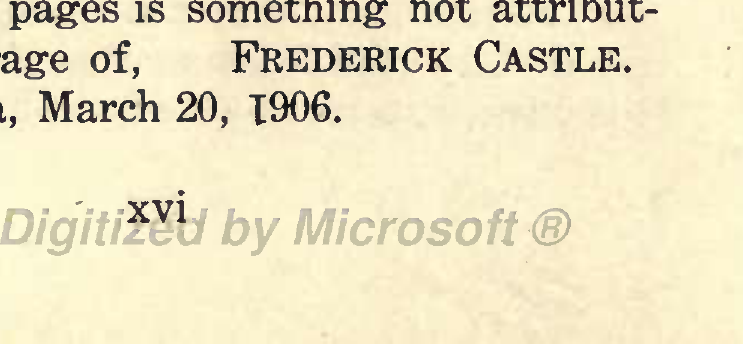
\includegraphics[width=0.8\textwidth]{../imagenes/pagina_024_fig_02.png}
\caption{Figura de la página 24}
\end{figure}

\begin{figure}[h!]
\centering
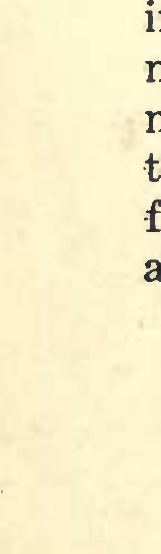
\includegraphics[width=0.8\textwidth]{../imagenes/pagina_024_fig_03.png}
\caption{Figura de la página 24}
\end{figure}

\begin{figure}[h!]
\centering
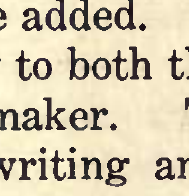
\includegraphics[width=0.8\textwidth]{../imagenes/pagina_024_fig_04.png}
\caption{Figura de la página 24}
\end{figure}

\begin{figure}[h!]
\centering
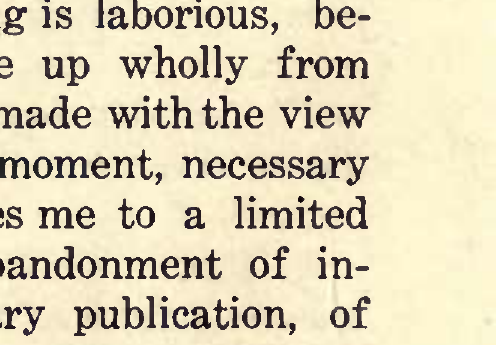
\includegraphics[width=0.8\textwidth]{../imagenes/pagina_024_fig_05.png}
\caption{Figura de la página 24}
\end{figure}

\begin{figure}[h!]
\centering
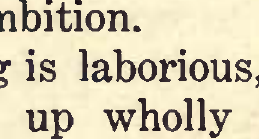
\includegraphics[width=0.8\textwidth]{../imagenes/pagina_024_fig_06.png}
\caption{Figura de la página 24}
\end{figure}

\begin{figure}[h!]
\centering
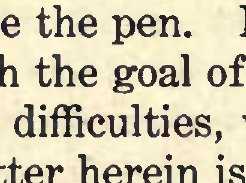
\includegraphics[width=0.8\textwidth]{../imagenes/pagina_024_fig_07.png}
\caption{Figura de la página 24}
\end{figure}

\begin{figure}[h!]
\centering
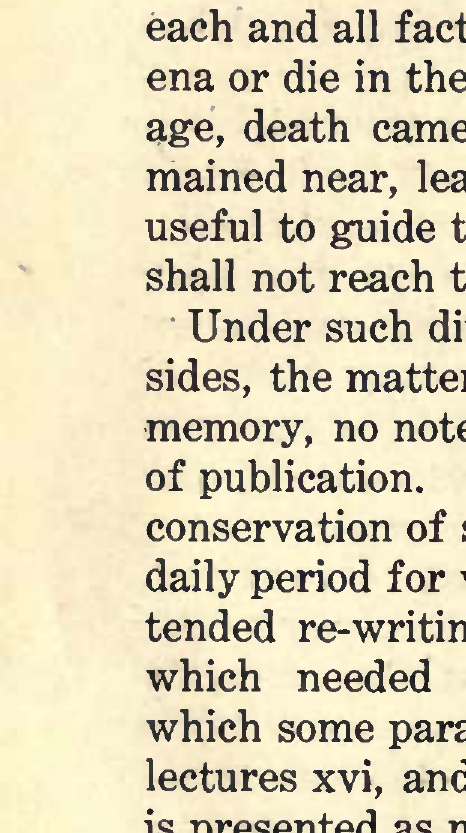
\includegraphics[width=0.8\textwidth]{../imagenes/pagina_024_fig_08.png}
\caption{Figura de la página 24}
\end{figure}

\begin{figure}[h!]
\centering
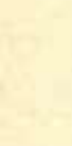
\includegraphics[width=0.8\textwidth]{../imagenes/pagina_024_fig_09.png}
\caption{Figura de la página 24}
\end{figure}

\begin{figure}[h!]
\centering
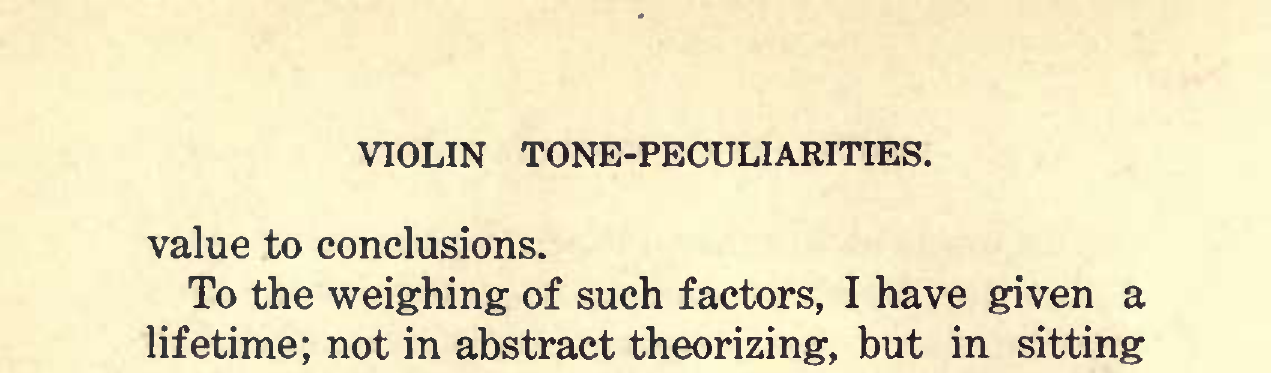
\includegraphics[width=0.8\textwidth]{../imagenes/pagina_024_fig_10.png}
\caption{Figura de la página 24}
\end{figure}

\section{VIOLIN TONE-PECULIARITIES.}

value to conclusions. To the weighing of such factors, I have given a lifetime; not in abstract theorizing, but in sitting at the bench while repeating demonstration after demonstration, year after year, decade after de- cade, from youth to old age, determined upon iso- lating, weighing, and knowing the operation of each and all factors underlying violin tone-phenom- ena or die in the attempt. At sixty-three years of age, death came near, and three years later re- mained near, leaving but my right arm sufficiently useful to guide the pen. It is now certain that I shall not reach the goal of my ambition. Under such difficulties, writing is laborious, be- sides, the matter herein is made up wholly from memory, no notes having been made with the view of publication. At the present moment, necessary conservation of strength confines me to a limited daily period for work; hence abandonment of in- tended re-writing of preliminary publication, of which needed corrections are made, and from which some paragraphs are omitted, and to which lectures xvi, and xvii, are added. This publication is presented as my legacy to both the violin student and the American violin maker. That the follow- ing record is reduced to writing and published is matter wholly due to encouragement offered by a modern violin maker; therefore, whatever of en- tertainment, or whatever of other value may be found upon these pages is something not attribut- able alone to courage of, FREDERICK CASTLE. Lowell, Indiana, March 20, 1906.

\section{xvi}

\begin{figure}[h!]
\centering
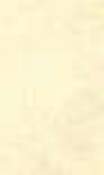
\includegraphics[width=0.8\textwidth]{../imagenes/pagina_025_fig_01.png}
\caption{Figura de la página 25}
\end{figure}

\begin{figure}[h!]
\centering
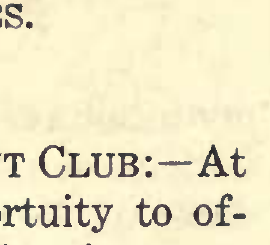
\includegraphics[width=0.8\textwidth]{../imagenes/pagina_025_fig_02.png}
\caption{Figura de la página 25}
\end{figure}

\section{VIOLIN TONE-PECULIARITIES.}

LECTURE I. GENTLEMEN OF THE VIOLIN STUDENT CLUB: At this, our first session, I take the opportuity to of- fer you congratulations for the following interest- ing facts. First: The causes for noisy violin tone are discovered. Second: A successful way to pre- serve interior surfaces of the violin from disinte- gration by heat and moisture has been perfected. Third: Areas of the violin sounding-board, re- sponsible for production and augmentation of tone are now located and defined. Fourth: A method for sounding-board graduation, securing maximum evenness of tone-power has received demonstration. Sixth: Principles, governing violin tone-intensity, are brought out into the light. Seventh: Princi- ples governing violin tone-power are reduced to words. Eighth: Quality of sounding-board wood, permitting ' 'rich ' ' violin tone, is described. Ninth : The power of accident to dispel darkness and de- lusion is placed on record. Tenth: Some scientific 'how conclusions concerning ' the violin operates to produce musical sound" have experienced a "jar." Eleventh: The fallacy in the claim that "the best of Cremonas are necessary vehicles for inter- pretation of Haydn, Mozart and Beethoven scores" is made manifest. Twelfth An attempt has been made to right the wrongs heaped : upon the modern violin maker by the "old- violin-trade-promoter. " During our course of study, you may be present- ed with some ideas pertaining to violin tone hereto- f ore" not given expression. Indeed, I promise you but little stale hash in our menu. As it is not

17

\section{VIOLIN TONE-PECULIARITIES.}

my intention to rob you of the pleasure afforded by anticipation, therefore you will be given but small doses at one time. This plan is adopted to avoid injuring your digestive power, and, to secure your regular attendance. Tone taste varies varies up through every de- gree of musical culture. A tone suiting one may in no wise suit another. No player can play his, or her, best upon an instrument whose tone to him, or her, is disagreeable. Fortunately, the violin affords a variety in tone-quality so infinitely great that every violin player on earth may own one having tone-quality to his taste. One might think it possible to make violins hav- ing a single standard of tone-quality, but the fact is, inherent peculiarity of action in wood stands in the way. There is something approaching an unvarying tone-standard for the whole range of wind instru- ments and instruments of percussion. But unvarying tone-quality suddenly halts in the presence of the violin family. We can imagine the unbounded surprise of one who never heard other than wind musical instruments upon introduction to this violin family. As he picks up violin after violin, viola after viola, cello after cello, he finds no two possessing an identical tone-character. Each violin, each viola, each cello, has a tone-qual- ity peculiar to itself. These peculiarities are so marked that he soon becomes able to name each violin with whose tones he is familiar, although blindfolded, or in a distant apartment, naming

18
